% !TeX root = ../../Skript.tex
\cohead{\Large\textbf{Hauptform}}
\fakesubsection{Hauptform}
Liegt die Funktionsgleichung einer quadratischen Funktion in der folgenden Darstellungsform vor, so spricht man von der Hauptform oder Normalform:
\begin{tcolorbox}\centering
	\(\textcolor{loestc}{f(x)=ax^2+bx+c, \quad a\neq 0}\)
\end{tcolorbox}

\begin{itemize}
    \setlength{\qrheight}{2.5cm}%
	\item Streckfaktor \(a\):
    \adjustbox{valign=t}{\begin{minipage}{0.635\textwidth+\qrheight}\adjustbox{valign=t}{\begin{minipage}{\textwidth-\qrheight}%
    \vspace{0.80ex}
    \textcolor{loes}{Gibt an, ob die Parabel schmaler \(\left(-1<a<1\right)\) oder breiter  \((a<-1\) oder \(a>1)\) als die Normalparabel ist und ob die Parabel nach oben (\(a\) positiv) oder nach unten (\(a\) negativ) geöffnet ist.}
    \end{minipage}}%
    \adjustbox{valign=t}{\begin{minipage}{\qrheight}%
    \iftoggle{qrcode}{%
            \href{https://www.geogebra.org/m/hnypxj99}{
\includegraphics[width=\qrheight]{\quadFkt/pics/HauptformQR.png}}%
    }{}%
    \end{minipage}}\end{minipage}}%

    \bigskip

	\item Koeffizient \(b\): \textcolor{loes}{Verschiebt die Parabel gleichzeitig in \(x\)-Richtung und \(y\)-Richtung.}

	\bigskip

	\item Absolutglied \(c\): \textcolor{loes}{Gibt den \(y\)-Achsenabschnitt an \(\left(f(0)=a\cdot 0^2+b\cdot 0+c=c\right)\).}

	\bigskip

\end{itemize}
Die Nullstellen einer quadratischen Funktion bzw. die Lösungen einer Gleichung vom Typ
\[{\textcolor{red}{a}x^2+\textcolor{blue}{b}x+\textcolor{ForestGreen}{c}=0}\]%

lassen sich mit Hilfe der Mitternachtsformel bestimmen:
\begin{tcolorbox}
\textbf{Mitternachtsformel}
\[x_{1/2}=\frac{-\textcolor{blue}{b}\pm\sqrt{\textcolor{blue}{b}^2-4 \textcolor{red}{a}  \textcolor{ForestGreen}{c}}}{2 \textcolor{red}{a}}\]%
\end{tcolorbox}

Wie viele Lösungen die Gleichung hat, hängt vom Term unter der Wurzel, der sogenannten Diskriminanten \(D\) ab:
\(D=\textcolor{blue}{b}^2-4 \textcolor{red}{a}  \textcolor{ForestGreen}{c}\)

\bigskip

\begin{minipage}{\textwidth}
	\begin{minipage}{0.33\textwidth}
		\centering{\(\textcolor{blue}{b}^2-4 \textcolor{red}{a}  \textcolor{ForestGreen}{c}>0\)}

		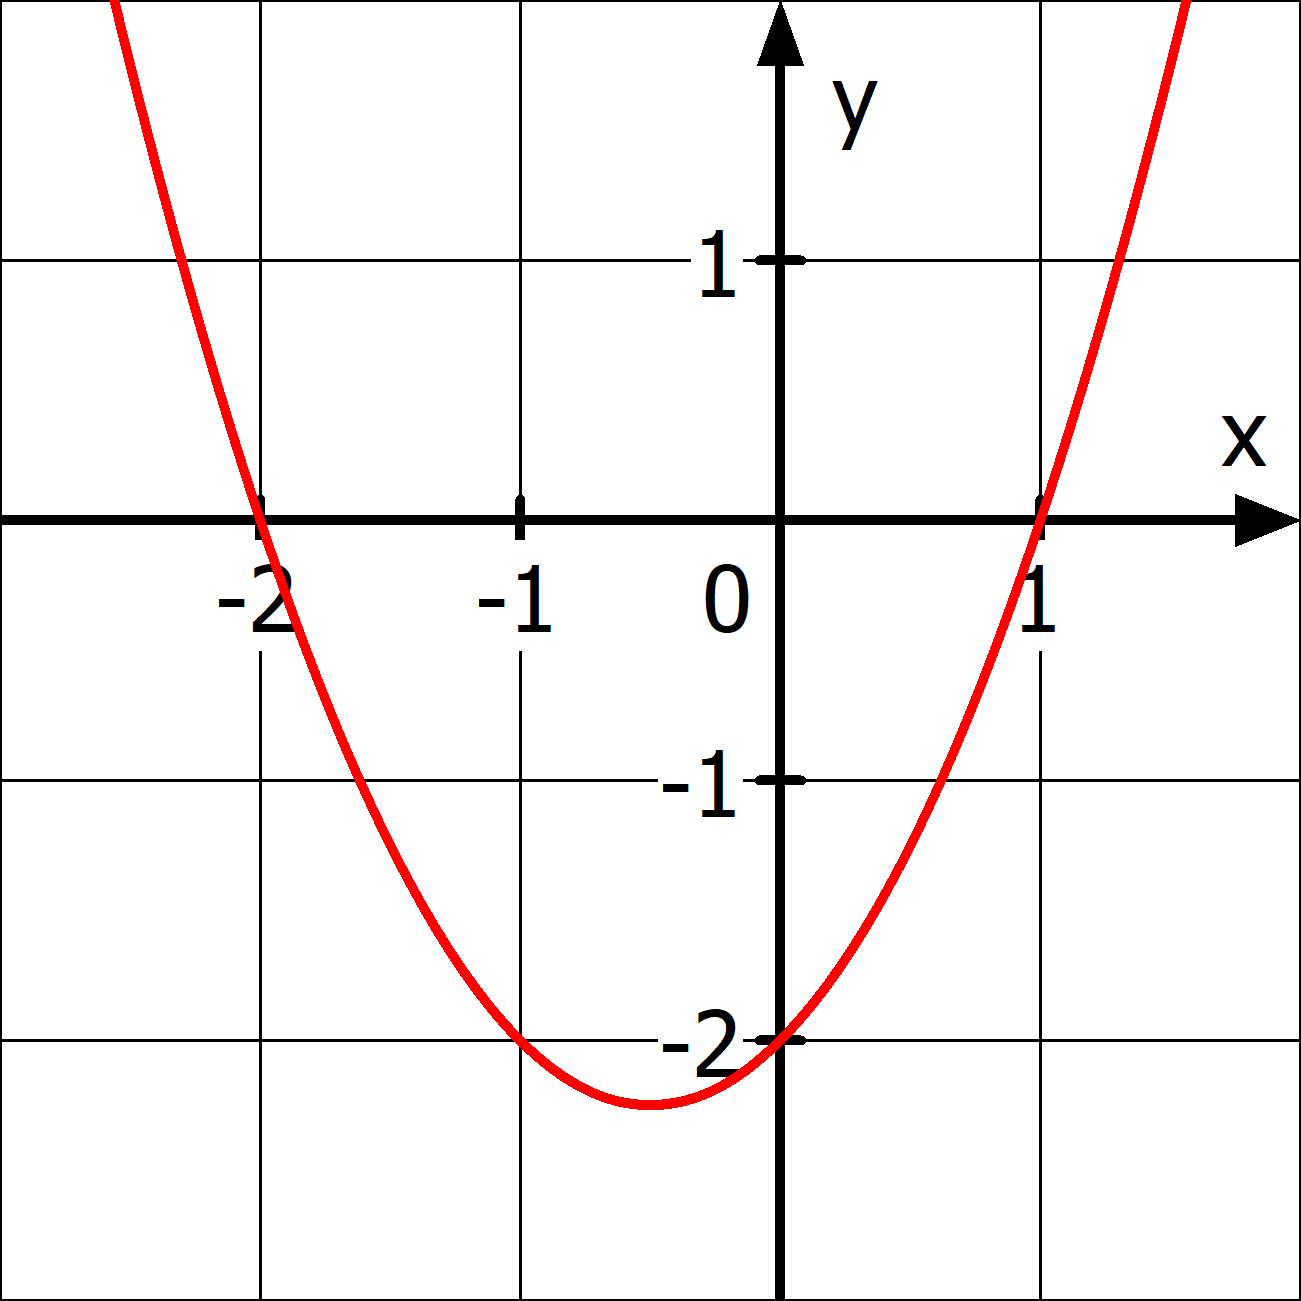
\includegraphics[width=.95\textwidth]{\quadFkt/pics/mitternacht2.png}

		\(f_1(x)=x^2+x-2\)
	\end{minipage}%
	\begin{minipage}{0.33\textwidth}
		\centering{\(\textcolor{blue}{b}^2-4 \textcolor{red}{a}  \textcolor{ForestGreen}{c}=0\)}

		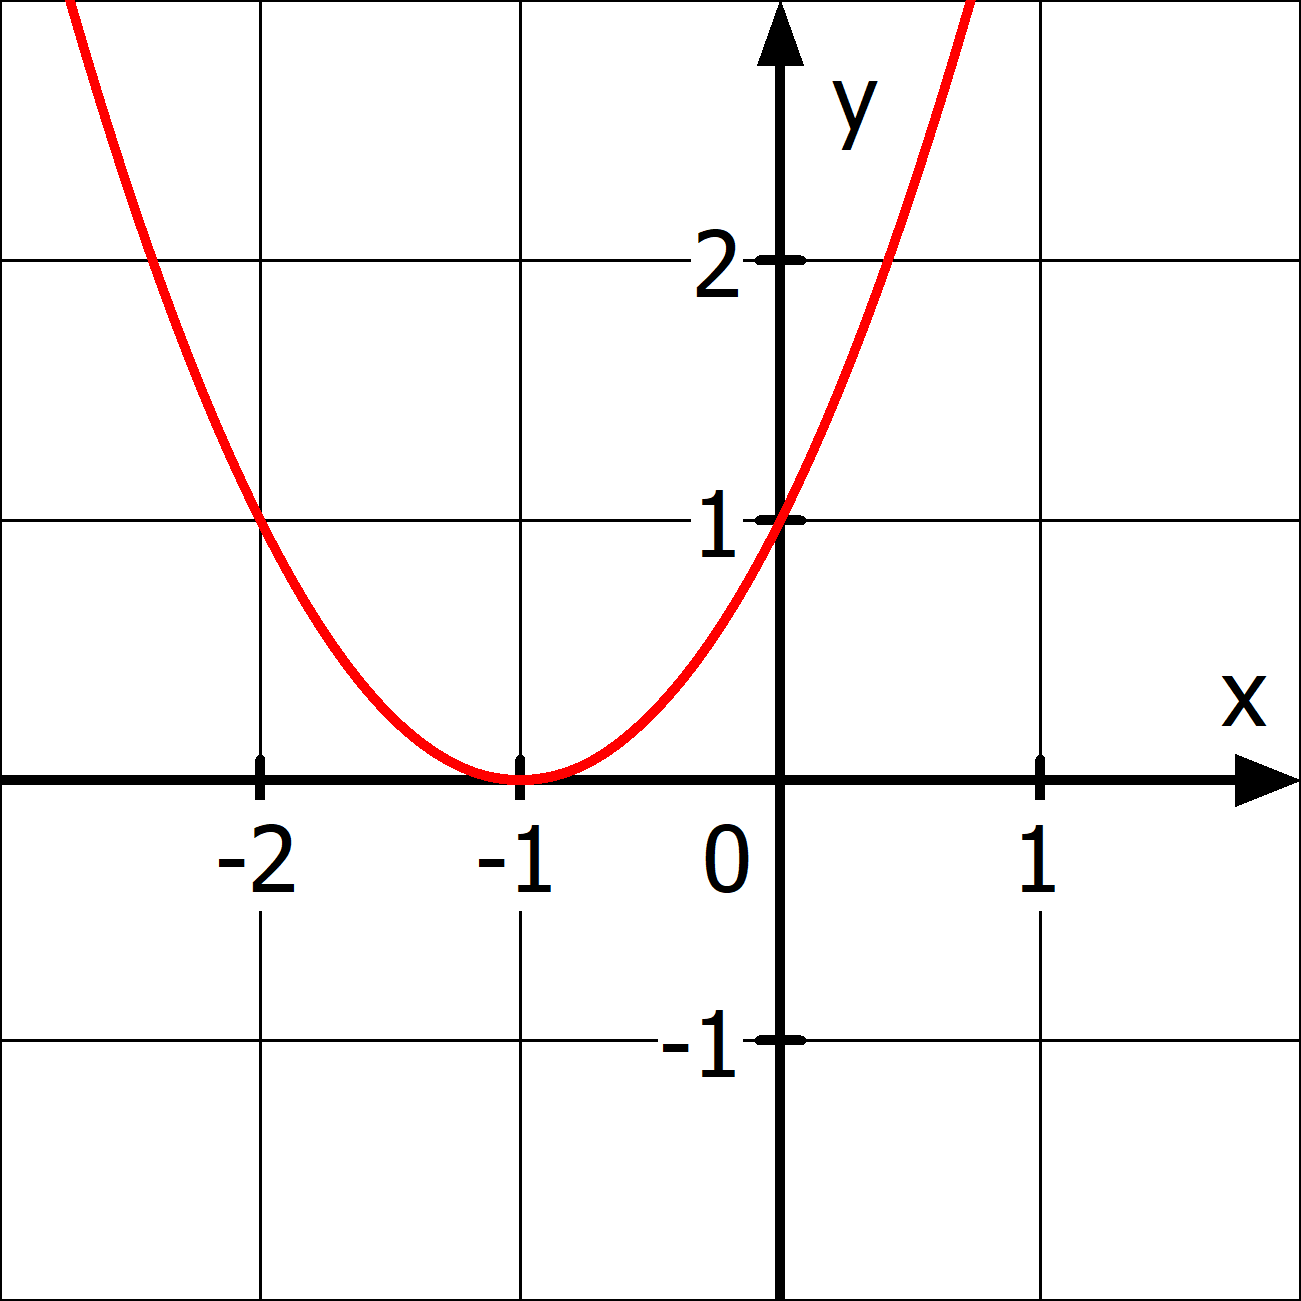
\includegraphics[width=.95\textwidth]{\quadFkt/pics/mitternacht1.png}

		\(f_2(x)=x^2-2x+1\)
	\end{minipage}%
	\begin{minipage}{0.33\textwidth}
		\centering{\(\textcolor{blue}{b}^2-4 \textcolor{red}{a}  \textcolor{ForestGreen}{c}<0\)}

		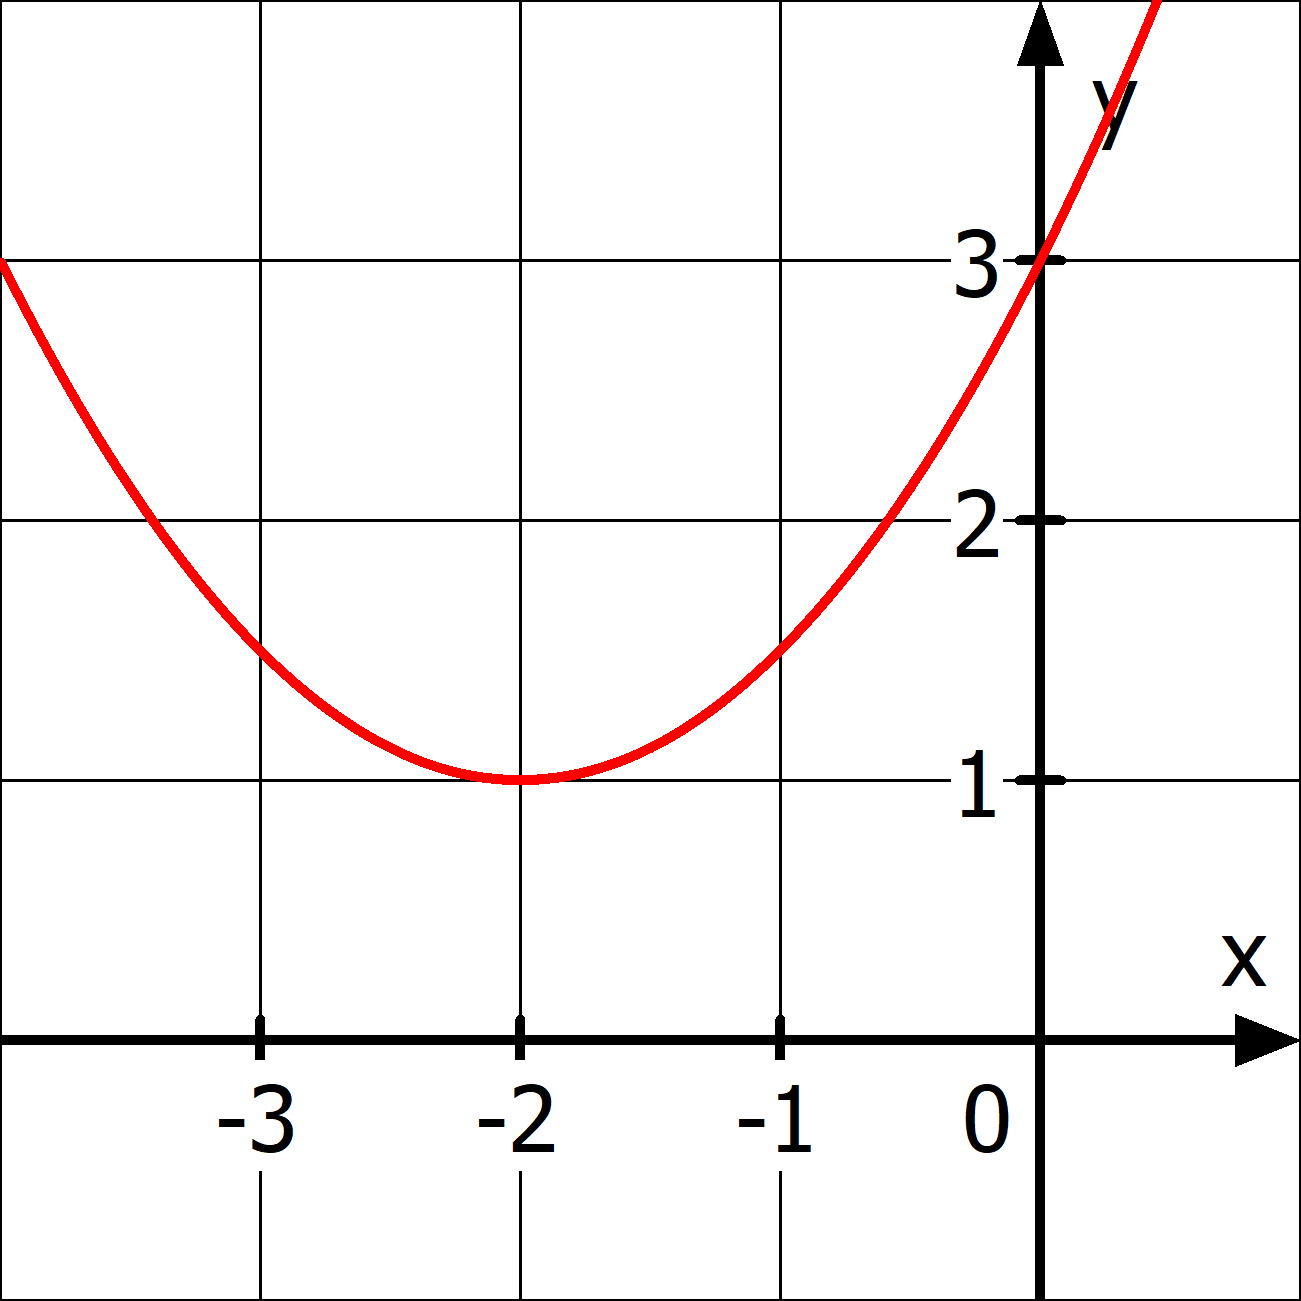
\includegraphics[width=.95\textwidth]{\quadFkt/pics/mitternacht0.png}

		\(f_3(x)=0,5x^2-2x+3\)
	\end{minipage}%
\end{minipage}

\bigskip

\begin{minipage}{\textwidth}
	\begin{minipage}{0.33\textwidth}
		\centering{\(\textcolor{loes}{x^2+x-2=0}\)}
	\end{minipage}%
	\begin{minipage}{0.33\textwidth}
		\centering{\(\textcolor{loes}{x^2+2x+1=0}\)}
	\end{minipage}%
	\begin{minipage}{0.33\textwidth}
		\centering{\(\textcolor{loes}{0,5x^2+2x+3=0}\)}
	\end{minipage}%
\end{minipage}

\bigskip

\begin{minipage}{\textwidth}
	\adjustbox{valign=t}{\begin{minipage}{0.33\textwidth}
		\color{loes}{\begin{align*}
				x_{1/2}&=\frac{-1\pm\sqrt{1^2-4\cdot 1\cdot (-2)}}{2\cdot 1}\\
				&=\frac{-1\pm 3}{2}\\
				x_1&=-2\quad x_2=1
		\end{align*}}
	\end{minipage}}%
	\adjustbox{valign=t}{\begin{minipage}{0.33\textwidth}
		\color{loes}{\begin{align*}
				x_{1/2}&=\frac{-2\pm\sqrt{2^2-4\cdot 1\cdot 1}}{2\cdot 1}\\
				&=\frac{-2\pm 0}{2}\\
				&=-1
		\end{align*}}
	\end{minipage}}%
	\adjustbox{valign=t}{\begin{minipage}{0.33\textwidth}
		\color{loes}{\begin{align*}
				x_{1/2}&=\frac{-2\pm\sqrt{2^2-4\cdot 0,5\cdot 3}}{2\cdot 0,5}\\
				&=-2\pm\sqrt{-2}\quad \Lightning
		\end{align*}}
	\end{minipage}}%
\end{minipage}
\newpage
%%%%%%%%%%%%%%%%%%%%%%%%%%%%%%%%%%%%%%%%%

\begin{Exercise}[title={Bestimme die Nullstellen}, label=normalformNullstellenA1]

	\begin{minipage}{\textwidth}
		\begin{minipage}{0.49\textwidth}
			\begin{enumerate}[label=\alph*)]
				\item \(f(x)=x^2+3x-4\)
				\item \(f(x)=x^2-4x+3\)
				\item \(f(x)=\frac{1}{2}x^2+\frac{5}{2}x+3\)
				\item \(f(x)=0,25x^2+x+1\)
				\item \(f(x)=-2x^2+4x-4\)
				\item \(f(x)=\frac{1}{3}x^2-x-6\)
				\item \(f(x)=0,1x^2-0,2x-1,5\)
			\end{enumerate}
		\end{minipage}
		\begin{minipage}{0.49\textwidth}
			\begin{enumerate}[label=\alph*)]
				\setcounter{enumi}{7}
				\item \(f(x)=2x^2-4x-2\)
				\item \(f(x)=\frac{1}{16}x^2-\frac{1}{4}x-2\)
				\item \(f(x)=0,5x^2+2x+0,5\)
				\item \(f(x)=\frac{2}{3}x^2+4x-18\)
				\item \(f(x)=0,25x^2-1,5x+1\)
				\item \(f(x)=4x^2+12x+13\)
				\item \(f(x)=0,2x^2-2x+5\)
			\end{enumerate}
		\end{minipage}
	\end{minipage}
\end{Exercise}

\newpage
\begin{Answer}[ref=normalformNullstellenA1]

	\begin{minipage}{\textwidth}
		\begin{minipage}{0.49\textwidth}
			\begin{enumerate}[label=\alph*)]
				\item \(x_1=1,\quad x_2=-4\)
				\item \(x_1=1,\quad x_2=3\)
				\item \(x_1=-2,\quad x_2=-3\)
				\item \(x_{1/2}=-2\)
				\item keine Nullstellen
				\item \(x_1=-3,\quad x_2=6\)
				\item \(x_1=-3,\quad x_2=5\)
			\end{enumerate}
		\end{minipage}
		\begin{minipage}{0.49\textwidth}
			\begin{enumerate}[label=\alph*)]
				\setcounter{enumi}{7}
				\item \(x_{1/2}=1\pm\sqrt{2}\)
				\item \(x_1=8,\quad x_2=-4\)
				\item \(x_{1/2}=-2\pm\sqrt{3}\)
				\item \(x_1=3,\quad x_2=-9\)
				\item \(x_{1/2}=3\pm\sqrt{5}\)
				\item keine Nullstellen
				\item \(x_{1/2}=5\)
			\end{enumerate}
		\end{minipage}
	\end{minipage}
\end{Answer}